%%%%%%%%%%%%%%%%%%%%%%%%%%%%%%%%%%%%%%%%%%%%%%%%%%%%%%%%%%%%%%%%%%%%%%%%%%%%%%
%%Skeleton LaTeX file: double column format.
%%%%%%%%%%%%%%%%%%%%%%%%%%%%%%%%%%%%%%%%%%%%%%%%%%%%%%%%%%%%
%%REMEMBER THAT THERES IS AN EIGHT PAGE SIZE RESTRICTION
%%%%%%%%%%%%%%%%%%%%%%%%%%%%%%%%%%%%%%%%%%%%%%%%%%%%%%%%%%%%

%%% Sample file for ME Project Papers for Evaluation by Supervisor and Reader

\documentclass{article}

\usepackage{multicol}
\usepackage{graphicx}

\pagestyle{empty}
\setlength{\topmargin}{ 0.25in}
\setlength{\columnsep}{2.0pc}
\setlength{\headheight}{0.0in}
\setlength{\headsep}{0.0in}
\setlength{\oddsidemargin}{-.19in}
\setlength{\parindent}{1pc}
\textheight 8.75in
\textwidth 6.8in

\title{\large \bf Predicting Query Execution Time }
\author{Name}

\date{}

\begin{document}

	\maketitle
    \begin{center}
        Mid-term ME Project Report
    \end{center}
        \vskip 12pt
	\thispagestyle{empty}
	\bibliographystyle{unsrt}
		\begin{abstract}
		The ability to estimate the query execution time is central for a number of tasks in database system
		such as query scheduling, progress monitoring and costing during query optimization. Recent work 
		has explored the use of statistical techniques in place of the manually constructed cost models used 
		in query optimization. Such techniques, which require as training data along with the 
		actual execution time, promises superior accuracies for they being able to account the for factors 
		such as hardware characteristics and bias in cardinality estimates. However, such techniques fail 
		to generalize i.e., produce poor estimates for queries that are not seen during the training.
		
		In this work, we propose and evaluate predictive modeling techniques that learn query 
		execution behavior at a fine grained operator level. For each operator, we consider different sets 
		of features and build different models for them. Since there are only finitely many operators in 
		database, this approach is practical and will be able to estimate any query as its a composition of
		many operators. We evaluate our approaches using TPC-H and TPC-DS workloads on PostgreSQL.

	\end{abstract}	
	
	\hfill \\
	
	\begin{multicols}{2}
	\section{INTRODUCTION}
	Database systems can greatly benefit from accurate execution time predictions including: 
	
	\begin{itemize}
	\item Query Optimizer: 
	\item Query Scheduling:
	\item Progress monitoring:
	\end{itemize}
	
	1D regression using linear, polynomial and RBF kernels.
	
	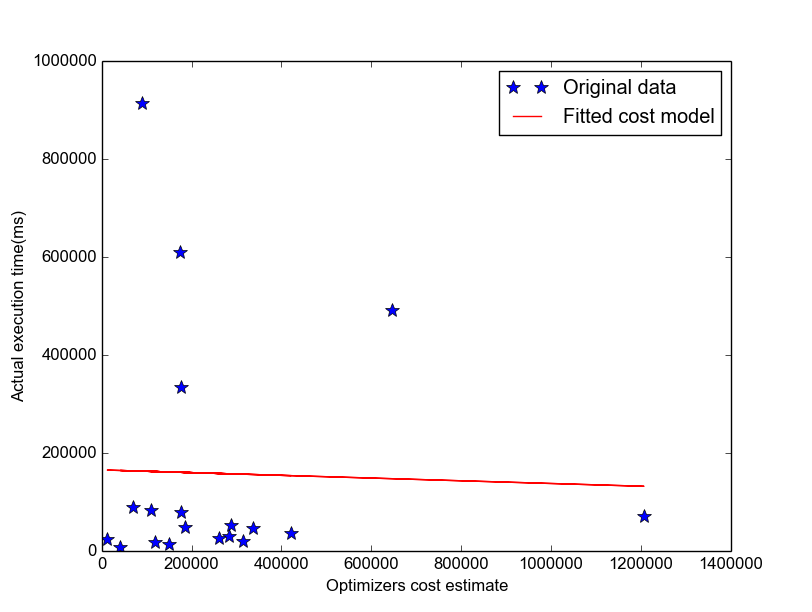
\includegraphics[scale=.33]{figure_1.png} 
		
	\section{2nd SECTION TITLE}
Pellentesque id leo eu massa rhoncus consectetur sit amet vel dui. Duis metus nibh, dignissim sit amet urna at, consequat semper libero. Fusce condimentum tortor mi, vel molestie sapien vehicula vitae. Integer ac ipsum sapien. Mauris lectus dolor, porta eget efficitur ac, varius a nulla. Fusce posuere dui ac nunc euismod, vitae convallis quam volutpat. Maecenas consequat malesuada porta. Nunc sit amet metus eget felis elementum porta. In eu vestibulum metus. Curabitur sed cursus purus.

%%%%%%%%%%%%%  This can be followed by several other sections

	\section{Conclusions and Future Work}
	Proin id elit nec erat pellentesque gravida ut a lectus. Proin rhoncus eu justo et aliquet. Praesent auctor augue quis magna dapibus imperdiet. Fusce vehicula vehicula aliquet. Fusce ac dolor in lorem tristique bibendum eget finibus turpis. In odio dui, mattis sed commodo non, bibendum et augue. Nam dignissim id metus ut bibendum. Nulla eu leo sed dui venenatis viverra. Donec et enim rutrum lorem aliquam bibendum ac ac arcu. Lorem ipsum dolor sit amet, consectetur adipiscing elit. In gravida enim vitae nisi tincidunt pulvinar. Maecenas hendrerit lacinia dui, et egestas turpis suscipit sed. Vestibulum eros orci, bibendum in diam in, suscipit aliquet ipsum. Nulla facilisi. Vestibulum vulputate, nulla ut ornare varius, eros leo elementum sem, at tempor ante massa vitae dolor.	
	
    \bibliographystyle{abbrv}
    \bibliography{}
	
	\end{multicols}
\end{document}
